\documentclass[11pt]{article}

% parameters are fairly self-explanatory here, thankfully
\usepackage[width=7in,height=9.5in,top=0.75in,centering]{geometry}

% for math-ing
\usepackage{amsmath}
\usepackage{amssymb}
\usepackage{comment}

%%%%%% tables %%%%%%%%
\usepackage{tabularx}
\usepackage{array}
\renewcommand{\arraystretch}{1.5}
\setlength{\tabcolsep}{8pt}

%%%%%% plotting %%%%%%

\usepackage[dvipsnames]{xcolor}
\usepackage{tikz}
\usepackage{pgfplots}

\pgfplotsset{every axis/.append style={
                    axis x line=middle,    % put the x axis in the middle
                    axis y line=middle,    % put the y axis in the middle
                    axis line style={<->,color=black}, % arrows on the axis
                    xlabel={$x$},          % default put x on x-axis
                    ylabel={$y$},          % default put y on y-axis
            }}
            
 \pgfplotsset{compat=1.14} % sometimes, everything falls apart without this
 
 %\usepgfplotslibrary{fillbetween} %for shading between curves

%%%%%% commands %%%%%%

% exam heading; course name is first argument, exam information is second argument
\newcommand{\Heading}[2]{
    \fbox{
        {\Large\textbf{#1}}
        }
    \hfill
    \fbox{
        \begin{minipage}{0.2\textwidth}
            \begin{center}
            \textbf{#2}
            \end{center}
        \end{minipage}
    }
    \par\vspace{0.1in}}

% for being lazy while beautifying integrals
\newcommand{\dint}{\displaystyle\int}

% for being lazy while beautifying limits
\newcommand{\dlim}{\displaystyle\lim}

%%%%%% stuff %%%%%%

\usepackage{fancyhdr}

%\setcounter{page}{0} % first page is page 0

\parindent0pt % no indent

\fboxsep=0.25cm % little space in fbox border

%%%%%% BEGIN! %%%%%%%

\begin{document}

\pagestyle{fancy}

% record goals here to create sense of transparency

\fancyhead[l]{%
  \ifcase\value{page}
  % empty test for page = 0
  \or {\bf\color{ProcessBlue} F1: Lines \& Slope}% page=1
  \or {\bf\color{RoyalBlue} L1: Limits and Continuity}% page = 2
  \or {\bf\color{RoyalBlue} L2: Evaluating Limits Using Continuity and Forms}% page = 3
  \or {\bf\color{ForestGreen} D1: Meaning of a Derivative}% page = 4
  \or
  \else
  % Empty chead here!
  \fi
}

% \thispagestyle{empty} % don't display that this is page 0

\Heading{MATH 1210}{Review Session 1\\Spring 2026\\
Section 930}

\vspace{0.1in}

\textbf{Name} \hrulefill
% \newpage%
%%%%%%%%%


\begin{enumerate}

%%%%%%%%%%%%%%%%%%%%%%%%%%%%%%%%%%%%%%%%%%%%%%%%%%%%%
%%%%%%%%%%% BEGIN PROBLEM F1 %%%%%%%%%%%%%%%%%%%%%%%%
%%%%%%%%%%%%%%%%%%%%%%%%%%%%%%%%%%%%%%%%%%%%%%%%%%%%%
\item[\textbf{F1}.]
The table below shows the relationship between the number of hours a server has been running
and the total amount of data processed by the server, measured in hundreds of gigabytes.

\begin{center}
\begin{tabular}{| l | c | c | c | c | c | c | c | c | c | c |}
% 0.5*pow(2,\x/2)
\hline
Time (hours) &
2 & 2.5 & 3 & 3.5 & 4 & 4.5 & 5 & 5.5 & 6 & 6.5 \\
\hline
Data processed (hundreds of GB) &
1 & 1.19 & 1.41 & 1.68 & 2 & 2.38 & 2.83 & 3.36 & 4 & 4.76 \\
\hline
\end{tabular}
\end{center}

\begin{enumerate}
    \item What is the average rate of change in data processed as the server runtime changes...

    \begin{enumerate}
    \item from $t=2$ hours to $t=6$ hours?
    \vfill
    \item from $t=2$ hours to $t=4$ hours?
    \vfill
    \end{enumerate}
    \textbf{Make sure to include units in your final result.}
    \vspace{.25in}

    \item Use a sentence or two to explain the meaning of the average rate of change on each of these intervals
    \textbf{in the context of this scenario}. 
    \begin{enumerate}
    \item
    % \vfill
    \item
    \vfill
    \end{enumerate}
    
    %Do NOT just say something vague like ``it is the average rate of change'' or ``it is the slope'' in your explanation.

    \vfill
\end{enumerate}


%%%%%%%%%%%%%%%%%%%%%%%%%%%%%%%%%%%%%%%%%%%%%%%%%%%%%
%%%%%%%%%%% END PROBLEM F1 %%%%%%%%%%%%%%%%%%%%%%%%%%
%%%%%%%%%%%%%%%%%%%%%%%%%%%%%%%%%%%%%%%%%%%%%%%%%%%%%

\newpage

%%%%%%%%%%%%%%%%%%%%%%%%%%%%%%%%%%%%%%%%%%%%%%%%%%%%%
%%%%%%%%%%% BEGIN PROBLEM L1 %%%%%%%%%%%%%%%%%%%%%%%%
%%%%%%%%%%%%%%%%%%%%%%%%%%%%%%%%%%%%%%%%%%%%%%%%%%%%%

\item[\textbf{L1}.]
Determine the types of discontinuity (if any)
together with the conditions they violate:

\begin{enumerate}
\item[(a)]
\noindent
\begin{minipage}[t]{0.4\textwidth}
\vspace{0pt}
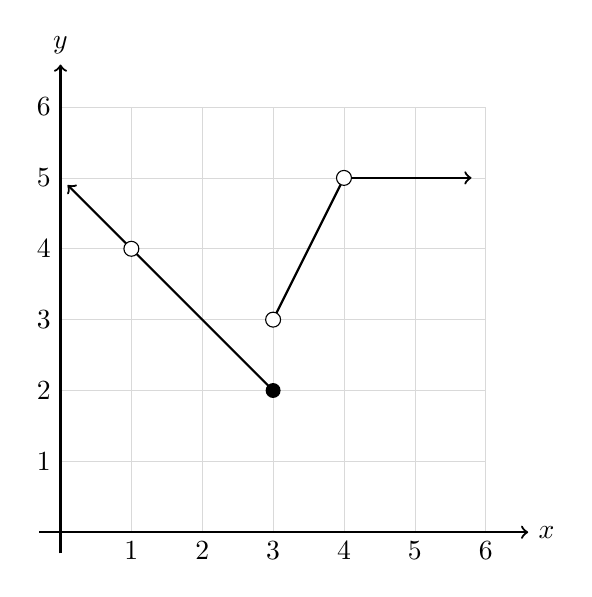
\begin{tikzpicture}[scale=0.9]
    % Grid
    \draw[step=1cm, gray!30, very thin] (0,0) grid (6,6);

    % Axes
    \draw[->, thick] (-0.3,0) -- (6.6,0) node[right]{$x$};
    \draw[->, thick] (0,-0.3) -- (0,6.6) node[above]{$y$};

    % Piecewise function with arrows
    \draw[thick, <-, domain=0.1:3] plot (\x, {5-\x});
    \draw[thick, domain=3.01:3.99] plot (\x, {2*\x-3});
    \draw[thick, ->, domain=4:5.8] plot (\x, {5});

    % Points
    \draw[fill=white] (1,4) circle (3pt);
    \fill (3,2) circle (3pt);
    \draw[fill=white] (3,3) circle (3pt);
    \draw[fill=white] (4,5) circle (3pt);

    % Tick labels
    \foreach \x in {1,2,3,4,5,6} \node[below] at (\x,0) {\x};
    \foreach \y in {1,2,3,4,5,6} \node[left] at (0,\y) {\y};
\end{tikzpicture}
\end{minipage}
\hspace{1em} % <-- controlled spacing instead of \hfill
\begin{minipage}[t]{0.40\textwidth}
\vspace{0pt}
\begin{tabular}{|c|c|c|}
    \hline
    \textbf{$x$-value} & \textbf{condition(s) violated} & \textbf{type} \\
    \hline
     & & \\
     & & \\
     & & \\
     & & \\
     & & \\
     & & \\
     & & \\
     \hline
\end{tabular}
\end{minipage}
\vspace{.25in}
\item[(b)]
\noindent
\begin{minipage}[t]{0.4\textwidth}
\vspace{0pt}
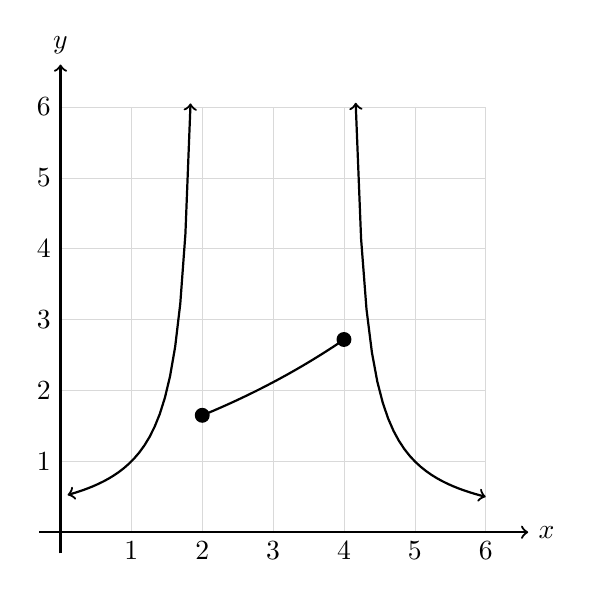
\begin{tikzpicture}[scale=0.9]
    % Grid
    \draw[step=1cm, gray!30, very thin] (0,0) grid (6,6);

    % Axes
    \draw[->, thick] (-0.3,0) -- (6.6,0) node[right]{$x$};
    \draw[->, thick] (0,-0.3) -- (0,6.6) node[above]{$y$};

    % Piecewise function with arrows
    \draw[thick, <->, domain=0.1:1.835] plot (\x, {1/(2-\x)});
    \draw[thick, domain=2:4] plot (\x, {e^(\x*0.25)});
    \draw[thick, <->, domain=4.165:6] plot (\x, {1/(\x-4)});

    % Points
    \fill (2,1.65) circle (3pt);
    \fill (4,2.72) circle (3pt);

    % Tick labels
    \foreach \x in {1,2,3,4,5,6} \node[below] at (\x,0) {\x};
    \foreach \y in {1,2,3,4,5,6} \node[left] at (0,\y) {\y};
\end{tikzpicture}
\end{minipage}
\hspace{1em} % <-- controlled spacing instead of \hfill
\begin{minipage}[t]{0.40\textwidth}
\vspace{0pt}
\begin{tabular}{|c|c|c|}
    \hline
    \textbf{$x$-value} & \textbf{condition(s) violated} & \textbf{type} \\
    \hline
     & & \\
     & & \\
     & & \\
     & & \\
     & & \\
     & & \\
     & & \\
     \hline
\end{tabular}
\end{minipage}

\vspace{.25in}
\item[(c)]
\noindent
\begin{minipage}[t]{0.4\textwidth}
\vspace{0pt}
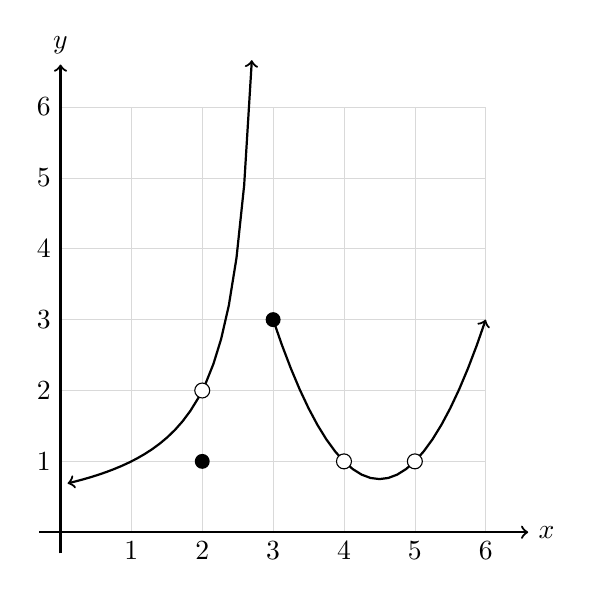
\begin{tikzpicture}[scale=0.9]
    % Grid
    \draw[step=1cm, gray!30, very thin] (0,0) grid (6,6);

    % Axes
    \draw[->, thick] (-0.3,0) -- (6.6,0) node[right]{$x$};
    \draw[->, thick] (0,-0.3) -- (0,6.6) node[above]{$y$};

    % Piecewise function with arrows
    \draw[thick, <->, domain=0.1:2.7] plot (\x, {2/(3-\x)});
    \draw[thick, ->, domain=3:6] plot (\x, {3+(\x-3)*(\x-6)});

    % Points
    \draw[fill=white] (2,2) circle (3pt);
    \fill (2,1) circle (3pt);
    \fill (3,3) circle (3pt);
    \draw[fill=white] (4,1) circle (3pt);
    \draw[fill=white] (5,1) circle (3pt);

    % Tick labels
    \foreach \x in {1,2,3,4,5,6} \node[below] at (\x,0) {\x};
    \foreach \y in {1,2,3,4,5,6} \node[left] at (0,\y) {\y};
\end{tikzpicture}
\end{minipage}
\hspace{1em} % <-- controlled spacing instead of \hfill
\begin{minipage}[t]{0.40\textwidth}
\vspace{0pt}
\begin{tabular}{|c|c|c|}
    \hline
    \textbf{$x$-value} & \textbf{condition(s) violated} & \textbf{type} \\
    \hline
     & & \\
     & & \\
     & & \\
     & & \\
     & & \\
     & & \\
     & & \\
     \hline
\end{tabular}
\end{minipage}
\end{enumerate}



%%%%%%%%%%%%%%%%%%%%%%%%%%%%%%%%%%%%%%%%%%%%%%%%%%%%%
%%%%%%%%%%% END PROBLEM L1 %%%%%%%%%%%%%%%%%%%%%%%%%%
%%%%%%%%%%%%%%%%%%%%%%%%%%%%%%%%%%%%%%%%%%%%%%%%%%%%%

\newpage

%%%%%%%%%%%%%%%%%%%%%%%%%%%%%%%%%%%%%%%%%%%%%%%%%%%%%
%%%%%%%%%%% BEGIN PROBLEM L2 %%%%%%%%%%%%%%%%%%%%%%%%
%%%%%%%%%%%%%%%%%%%%%%%%%%%%%%%%%%%%%%%%%%%%%%%%%%%%%

\item[\textbf{L2}.]
Evaluate the following limits using continuity or a specific form.

If you use continuity to evaluate a limit, please provide sufficient explanation for why continuity can be used, including why the given function is continuous at the given point.

If you use a form to evaluate a limit, please list the form and show all steps. 
\vspace{.25em}

\begin{enumerate}
    \item 
    \begin{tabularx}{\textwidth}{lX X}
        $\displaystyle \lim_{x\to 3} \frac{e^x+12}{\sqrt{x}-2}$ & 
        \textbf{Value:} \hrulefill & 
        \textbf{Form:} \hrulefill
    \end{tabularx}
    
    \vfill

    % 2. Hierarchy / finite value
    \item 
    \begin{tabularx}{\textwidth}{lX X}
        $\displaystyle \lim_{x\to \infty} \frac{7x^5 + 4x^4+x+9}{3x^5 - x^2}$ & 
        \textbf{Value:} \hrulefill & 
        \textbf{Form:} \hrulefill
    \end{tabularx}
    
    \vfill

    % 3. Limit goes to 0
    \item 
    \begin{tabularx}{\textwidth}{lX X}
        $\displaystyle \lim_{x\to \infty} \frac{x^4+3x^2+11}{-3^x + x}$ & 
        \textbf{Value:} \hrulefill & 
        \textbf{Form:} \hrulefill
    \end{tabularx}
    
    \vfill

    % 1. -c/0^+
    \item 
    \begin{tabularx}{\textwidth}{lX X}
        $\displaystyle \lim_{x\to 1} \frac{x^2 - 6}{x-1}$ & 
        \textbf{Value:} \hrulefill & 
        \textbf{Form:} \hrulefill
    \end{tabularx}

    \vfill
\end{enumerate}



%%%%%%%%%%%%%%%%%%%%%%%%%%%%%%%%%%%%%%%%%%%%%%%%%%%%%
%%%%%%%%%%% END PROBLEM L2 %%%%%%%%%%%%%%%%%%%%%%%%%%
%%%%%%%%%%%%%%%%%%%%%%%%%%%%%%%%%%%%%%%%%%%%%%%%%%%%%

\newpage

%%%%%%%%%%%%%%%%%%%%%%%%%%%%%%%%%%%%%%%%%%%%%%%%%%%%%
%%%%%%%%%%% BEGIN PROBLEM D1 %%%%%%%%%%%%%%%%%%%%%%%%
%%%%%%%%%%%%%%%%%%%%%%%%%%%%%%%%%%%%%%%%%%%%%%%%%%%%%
\item[\textbf{D1}.]
Network throughput $T$
measures the maximum amount of data a server can successfully transmit.
Throughput is measured in
Mbps (megabits per second),
that is, the amount of data delivered per unit time.
Network throughput can be regarded as a function
$T=g(N)$
of the number of active users 
$N$
connected to the server.
Typical values of 
$N$ under various conditions are shown below:
\begin{center}
\begin{tabular}{|l|l|}
\hline
\textbf{number of users $N$} & \textbf{conditions} \\
\hline
1 & single user \\
\hline
20 & small office \\
\hline
200 & medium organization \\
\hline
1000 & busy corporate network \\
\hline
5000 & peak traffic \\
\hline
20000 & overloaded system \\
\hline
\end{tabular}
\end{center}
\begin{enumerate}
\item[(a)]
What are the units of $g'(N)$?
\vfill
\item[(b)]
Assuming the server performs best under moderate load
(around 1000 users),
decide whether the following are positive, negative,
or zero:
\begin{enumerate}
    \item $g'(200)$
    \vspace{0.25in}
    \item $g'(1000)$
    \vspace{0.25in}
    \item $g'(5000)$
    \vspace{0.25in}
\end{enumerate}
% \vspace{0.25in}
(You may simply write your answers.)
% \vfill
\item[(c)]
Interpret the meaning of 
$g'(2000)$.
Write your answer in \textbf{the
context of the problem}.
\vfill
\end{enumerate}

\vfill
%%%%%%%%%%%%%%%%%%%%%%%%%%%%%%%%%%%%%%%%%%%%%%%%%%%%%
%%%%%%%%%%% END PROBLEM D1 %%%%%%%%%%%%%%%%%%%%%%%%%%
%%%%%%%%%%%%%%%%%%%%%%%%%%%%%%%%%%%%%%%%%%%%%%%%%%%%%
\end{enumerate}

\end{document}